\chapter{Módulo da Informação Visual} \label{chap:chap3}

Neste capítulo será introduzido o módulo de informação visual desenvolvido, sendo apresentadas a estrutura e organização deste sistema. Como referido no capítulo~\ref{chap:intro}, este projeto tem como objetivo estender a ferramenta TweeProfiles descrita na secção~\ref{sec:tweep}, dando-lhe uma dimensão de conteúdo diferente à que possui. Em conjunto com a informação espacial e temporal, O conteúdo das imagens partilhadas em tweets passa a ser uma fonte de informação e não o texto. Para que isto seja realizável, foi necessário o desenvolvimento de um módulo que efetue a recolha os dados com a devida filtragem, extraia e processe a informação visual e armazene essa informação de modo a que fosse possível a sua integração com o TweeProfiles. 

\section{Recolha dos Dados}\label{sec:dados}

O desenvolvimento deste módulo apenas era realizável com um conjunto de imagens partilhadas no serviço de microblogging Twitter, sendo fundamental a recolha dos dados necessários para esse processo, neste caso, os Tweets. Nesta secção é feita uma descrição do conjunto dos dados disponíveis, das filtragens que foram necessárias realizar e uma apresentação do conjunto de dados finais obtidos e utilizados no desenvolvimento deste projeto de dissertação.

\subsection{Descrição dos Dados}

O primeiro passo para a realização deste projeto de dissertação foi a recolha dos dados necessários. Estes dados foram recolhidos através de uma base de dados MongoDB previamente criada usando a plataforma Socialbus, anteriormente designada por TwitterEcho~\cite{Boanjak2012}. Este dados são estruturados sobre a forma de objetos JSON e possuem informação relativa a cada tweet. Estes objetos encontram-se todos num só documento MongoDB que se caracteriza pelas características apresentadas na Tabela~\ref{tab:nbrtweets}

\vspace{5 mm}
\begin{table}[h]
\centering
\begin{tabular}{|l|c|c|l|l|l|}
\hline
          & Total                        & Com imagem & Twitter                  & TwitPic                   & Instagram                  \\ \hline
Nº Tweets & \multicolumn{1}{r|}{1704273} & 86349      & \multicolumn{1}{c|}{202} & \multicolumn{1}{c|}{6100} & \multicolumn{1}{c|}{79210} \\ \hline
\end{tabular}
\caption{Descrição em números do total de tweets com indicação, nos que contém URL para imagem, do número de tweets por serviço de partilha de imagem}
\label{tab:nbrtweets}
\end{table}
\vspace{5 mm}

Estes tweets foram recolhidos entre o dia 17 e 19 de Junho de 2013 com conteúdo partilhado somente contendo texto escrito em português do Brasil, filtrados pela ferramenta Socialbus~\cite{Boanjak2012} já referida anteriormente. Estas datas coincidiram com um evento ocorrido no Brasil, mais especificamente, as manifestações do ano passado do povo brasileiro contra o seu governo. Este foi um dos motivos da escolha desta base de dados, pois apresentava tweets que poderiam ser interessante para encontrar padrões ou eventos através das imagens partilhadas pelos brasileiros nas ruas, aliadas sempre às dimensões espaço-temporais. 

\subsection{Filtragem dos Dados}

Após estar definido o conjunto de dados a utilizar, foi necessário realizar uma filtragem dos dados de modo a apresentarem a informação necessária para a realização deste projeto. O primeiro passo desta filtragem foi recolher todos os tweets que contivessem no seu objeto um URL para uma imagem, sendo que esse URL teria de pertencer a um dos seguintes serviços: 

\begin{itemize}
\item Twitter
\item TwitPic
\item Instagram
\end{itemize}
O URL teria que ser válido, isto é, foi feita uma verificação prévia se a imagem estaria ainda disponível através do endereço existente.

Para ser mais fácil posteriormente uma seleção mais cuidadosa dos tweets foi criada uma base de dados local (SQLite) com a seguinte tabela:

\begin{lstlisting}[language=SQL]
create table if not exists IMAGENS ( 
	id integer PRIMARY KEY AUTOINCREMENT, 
	id_tweet text, 
	servico text, 
	url text, 
	tipo text, 
	retweet text 
); 
\end{lstlisting}

Em que se descreve cada coluna da seguinte forma:

\begin{description}
\item[id] - id da linha da tabela;
\item[id\_tweet] - id do tweet na base de dados Mongodb;
\item[servico] - nome do serviço de alojamento da imagem;
\item[url] - endereço url para a imagem fonte;
\item[tipo] - este atributo identifica se a imagem pertence a um tweet ou retweet;
\item[retweet] - caso a imagem pertença a um retweet, este atributo pode assumir o valor "primeiro" no caso de ser o primeiro retweet, do tweet original, na base de dados MongoDB, ou caso contrário, assume o valor NULL.
\end{description}

Isto permitiu realizar de uma forma rápida alguns teste no \textit{download} de algumas imagens pelos diferentes serviços, para além de permitir fazer uma seleção fácil e rápida de tweets, retweets ou por exemplo, do primeiro retweet no caso de existir vários retweets de um determinado tweet. 

Após a criação desta base de dados, ficou decidido selecionar todos os objetos da base de dados MongoDB do tipo tweet em que o seu serviço fosse o Instagram. Esta decisão deveu-se ao facto dos retweets se referirem a imagens já existentes ocorrendo duplicação de dados. No caso da escolha do Instagram, este deveu-se ao facto de apresentar um número superior de imagens relativamente aos outros serviços, visto que ao se excluir os retweets o número de imagens dos restantes serviços passou a um valor pouco significativo.

Para além destes critérios é importante salientar que foi necessário selecionar apenas os dados com georreferenciação. 

\subsection{Conjunto de Dados Final}

Por fim armazenou-se um ficheiro JSON com todos os dados que serão utilizados e foi realizado o \textit{download} de todas as imagens relativas a cada tweet e armazenadas localmente em formato JPEG, que se apresentava como formato de origem das imagens descarregadas. 

Relativamente aos objetos de cada tweet presentes no ficheiro JSON, optou-se por não armazenar todas as instâncias para reduzir o tamanho do ficheiro, tendo sido apenas incluídas as representadas no seguinte exemplo de um objeto de um tweet:

\lstinputlisting[language=Python]{./code/tweets_instagram_exemple.json}

No caso das imagens armazenadas, de modo a que fosse associada cada uma das imagens ao seu respetivo tweet, foi atribuído o campo \textit{id\_str} presente no objeto JSON ao nome do ficheiro de imagem JPEG. Assim ao utilizar uma das imagens, para saber a que tweet pertence apenas é necessário procurar o objeto JSON que possua o atributo \textit{id\_str} igual ao nome do ficheiro da imagem.

Recolhidos todos os identificadores dos tweets pertencentes ao serviço Instagram que apenas fossem do tipo tweet e que os respetivos tweets apresentassem a informação de geolocalização no campo \textit{coordinates}, avançou-se com o processo de \textit{download} de todas as imagens, tendo sido efetuado com sucesso o \textit{download} de 5964 imagens em 7195 possíveis.

Em suma, o conjunto de dados final utilizado para o desenvolvimento deste projeto foi de 5964 objetos relativos aos tweets contidos num ficheiro JSON e as respetivas 5964 imagens.

\section{Extração, Processamento e Armazenamento da Informação Visual} \label{sec:extract}

O passo seguinte no desenvolvimento do módulo da informação visual foi a implementação de um sistema capaz de extrair, processar e armazenar a informação visual através das imagens armazenadas localmente. Para o desenvolvimento deste modulo foi utilizada a linguagem Python, pela sua capacidade de integração de diferentes bibliotecas desde manipulação de estruturas de dados, até mesmo a bibliotecas de manipulação e processamento de imagem. Para a concretização do modelo foram tidos como linhas guia, o processo desenvolvimento de uma ferramenta de pesquisa de imagens apresentado em~\cite{Solem2012}. A arquitetura deste módulo desenvolvido é apresentada na Figura~\ref{fig:infovisual}.

\begin{figure}[h]
\centering
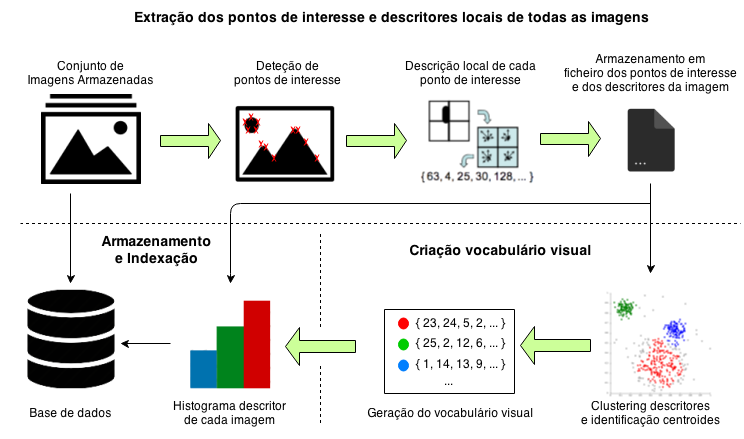
\includegraphics[width=0.95\linewidth]{./figures/infovisual}
\caption{Arquitetura do módulo de extração, processamento e armazenamento da informação visual. \textit{Adaptada de}~\cite{Bueno2011}}
\label{fig:infovisual}
\end{figure}

Foram desenvolvidos três sub-módulos diferentes: o primeiro é responsável pela extração dos descritores locais, o segundo utiliza o primeiro para gerar um vocabulário visual, e o terceiro utiliza os dois anteriores para armazenar um histograma descritor de cada imagem numa base de dados indexada à sua respetiva imagem. 
Em seguida é apresentada uma subsecção com a descrição para cada sub-módulo, como representado na Figura~\ref{fig:infovisual}

\subsection{Extração dos Pontos de Interesse e Descritores Locais}

O primeiro passo no desenvolvimento deste módulo passou pela extração da informação visual. Esta informação visual deveria representar uma imagem eficientemente e de forma a possibilitar a criação de um vocabulário visual. Uma das formas possíveis e apresentadas na secção~\ref{sec:represent} é a utilização de um descritor local. Neste caso foi utilizado o descritor SIFT~\cite{Lowe1999, Lowe2004}, pois como referido na secção~\ref{subsec:desclocal}, apesar de ser mais lento e menos eficiente a mudanças de iluminação, este apresenta melhores resultados a variações de rotação, mudanças de escala e transformações na imagem. Para além disso, foi utilizada a ferramenta e biblioteca \textit{open source} VLFeat~\cite{vedaldi08vlfeat} que integra alguns dos algoritmos mais utilizados em visão computacional, e que inclui o algoritmo SIFT. Este, apesar de não possuir uma biblioteca para Python, permite a sua utilização através da linha de comandos.

Para o conjunto de imagens existentes foi necessário criar uma cópia de cada imagem em escalas de cinzento e em formato \textit{.pgm} para ser utilizada pelo VLFeat. Utilizando assim estas imagens, o VLFeat armazena num ficheiro com o formato \textit{.sift} os pontos de interesse e os descritores de uma imagem, sendo necessário criar um ficheiro para cada imagem. Nesses ficheiros os dados são armazenados em formato ASCII. 
A informação armazenada apresenta-se da seguinte forma 

\begin{lstlisting}
318.861 7.48227 1.12001 1.68523 0 0 0 1 0 0 0 0 0 11 16 0 ...
318.861 7.48227 1.12001 2.99965 11 2 0 0 1 0 0 0 173 67 0 0 ...
54.2821 14.8586 0.895827 4.29821 60 46 0 0 0 0 0 0 99 42 0 0 ...
155.714 23.0575 1.10741 1.54095 6 0 0 0 150 11 0 0 150 18 2 1 ...
42.9729 24.2012 0.969313 4.68892 90 29 0 0 0 1 2 10 79 45 5 11 ...
229.037 23.7603 0.921754 1.48754 3 0 0 0 141 31 0 0 141 45 0 0 ...
232.362 24.0091 1.0578 1.65089 11 1 0 16 134 0 0 0 106 21 16 33 ...
201.256 25.5857 1.04879 2.01664 10 4 1 8 14 2 1 9 88 13 0 0 ...
... ...
\end{lstlisting}

onde cada linha contêm as coordenadas, escala e ângulo de rotação para cada ponto de interesse, nos primeiros 4 valores respetivamente, correspondendo os restantes ao vetor descritor de tamanho 128 como referido na secção~\ref{subsec:desclocal}. Como o objetivo era utilizar as imagens originais, foram eliminadas as imagens temporárias com o formato \textit{.pgm}. O passo seguinte passou pelo desenvolvimento do submodelo responsável pela criação do vocabulário visual, que é apresentado na subsecção seguinte.

\subsection{Criação do Vocabulário Visual}

Este módulo é o responsável pela criação do vocabulário visual. Para a sua concretização foi necessário utilizar os ficheiros de extensão \textit{.sift} reproduzidos através da ferramenta VLFeat~\cite{vedaldi08vlfeat} no módulo anterior. 
%Os passos seguintes basearam-se nos descritos em~\cite{Solem2012}. 

As palavras visuais não são nada mais do que um conjunto de vetores de características de imagens. Assim um vocabulário visual é o conjunto destas palavras visuais. Como cada imagem possui muitos descritores locais, sendo que muitos podem ser semelhantes, é necessário agrupar todos os descritores de um conjunto de imagens e detetar aqueles que possam representar um conjunto de descritores semelhantes, e assim formar várias palavra visual, sendo uma palavra visual um centroide de um grupo.

Para criar um vocabulário visual foi então necessário utilizar um algoritmo de \textit{clustering} por partição, tendo sido escolhido o \textit{k-means} por ser um dos mais utilizados e eficiente, como foi referido na secção~\ref{subsec:parti}. O algoritmo foi aplicado aos descritores de um subconjunto de imagens aleatoriamente selecionadas do conjunto de imagens armazenadas localmente. Neste caso foi utilizado aproximadamente 8\% das imagens para não comprometer o tempo de processamento. Como este algoritmo implica a pré definição do número de \textit{clusters}, foi atribuído a \textit{k} o valor 1000. Isto significa que são gerados cerca de 1000 \textit{clusters}, ou seja, o nosso vocabulário visual possuirá cerca de 1000 palavras visuais.

\begin{figure}
\centering
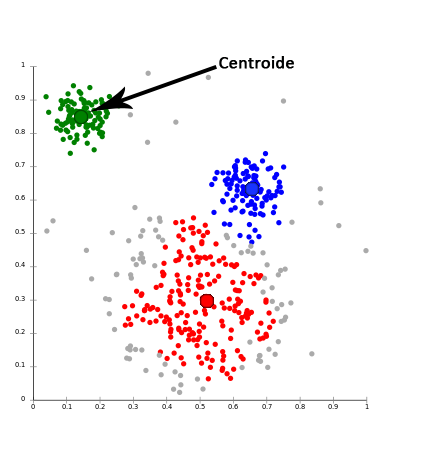
\includegraphics[width=0.6\linewidth]{./figures/centroides}
\caption{Exemplo de projeção de centroides após tarefa de \textit{clustering} num espaço a duas dimensões.}
\label{fig:centroides}
\end{figure}

Para utilizar este vocabulário visual é necessário armazená-lo e indexar cada palavra visual a cada imagem. O sub-módulo responsável por este processo é descrito na secção a seguir.

\subsection{Armazenamento da Informação Visual}

Com o vocabulário visual criado foi necessário armazenar esta informação e indexar cada palavra visual as imagens, de modo a que seja possível a comparação entre imagens diferentes. Para armazenar este vocabulário desenvolveu-se o módulo que execute esta tarefa, sendo que, foi necessário seguir alguns passos tais como, a criação de um histograma descritor do vocabulário visual de cada imagem e criação de uma base de dados com a informação necessária para a utilização do histograma descritor de cada imagem.

A criação do histograma foi o primeiro passo do desenvolvimento deste sub-módulo, em que foi utilizado o vocabulário disponibilizado através do sub-módulo apresentado anteriormente. Como o vocabulário é constituído por vetores descritores que representam cada uma das palavras visuais, para a criação do histograma para cada imagem foi necessário utilizar novamente os ficheiros com os descritores locais SIFT de cada imagem e assim projetar no espaço cada ponto-chave, de modo a ser atribuído a cada um destes a sua palavra visual, sendo esta a que se encontrar à menor distância. Foi então possível após este processo criar um histograma, utilizando  com a contagem das palavras visuais em cada imagem.

Assim o próximo passo passou pelo armazenamento dos histogramas e a indexação a sua respetiva imagem. Como todo este módulo foi operado em modo \textit{offline}, optou-se pela utilização de uma base de dados local SQLite~\cite{sqlite}. Esta funciona de modo semelhante a uma base de dados MySQL~\cite{mysql} ou PostgreSQL~\cite{postgresql}, sendo que pode ser desenvolvida e acedida sem recurso a um servidor. Para a sua concretização foi criado um esquema simples apenas com três tabelas como ilustrado na Tabela~\ref{tab:schemadb}. A tabela \textit{imlist} contém o nome de todas as imagens através do atributo \textit{filename}, a tabela \textit{imwords} contém índice das palavras visuais através do atributo \textit{wordid}, a identificação do vocabulário com o atributo \textit{vocname} e o índice das imagens em que as palavras visuais aparecem com o atributo \textit{wordid}. Por fim, a tabela \textit{imhistograms} contém o histograma de palavras visuais completo para cada imagem com o atributo \textit{histogram}.

%\vspace{2 mm}
\begin{table}[h]
\centering
\begin{tabular}{lcccc}
\multicolumn{5}{l}{} \\ \cline{1-1} \cline{3-3} \cline{5-5} 
\multicolumn{1}{|c|}{\cellcolor[HTML]{C0C0C0}\textbf{imlist}} & \multicolumn{1}{c|}{} & \multicolumn{1}{c|}{\cellcolor[HTML]{C0C0C0}\textbf{imwords}} & \multicolumn{1}{c|}{} & \multicolumn{1}{c|}{\cellcolor[HTML]{C0C0C0}\textbf{imhistograms}} \\ \cline{1-1} \cline{3-3} \cline{5-5} 
\multicolumn{1}{|c|}{rowid} & \multicolumn{1}{c|}{} & \multicolumn{1}{c|}{imid} & \multicolumn{1}{c|}{} & \multicolumn{1}{c|}{imid} \\ \cline{1-1} \cline{3-3} \cline{5-5} 
\multicolumn{1}{|c|}{filename} & \multicolumn{1}{c|}{\multirow{-3}{*}{}} & \multicolumn{1}{c|}{wordid} & \multicolumn{1}{c|}{} & \multicolumn{1}{c|}{histogram} \\ \cline{1-1} \cline{3-3} \cline{5-5} 
 & \multicolumn{1}{l|}{} & \multicolumn{1}{c|}{vocname} & \multicolumn{1}{c|}{\multirow{-4}{*}{}} & \multicolumn{1}{c|}{vocname} \\ \cline{3-3} \cline{5-5} 
\multicolumn{5}{l}{}
\end{tabular}
\caption{Esquema da base de dados SQLite}
\label{tab:schemadb}
\end{table}

\section{Matriz de Distâncias entre Imagens}\label{sec:matdist}

Com o módulo descrito na secção anterior~\ref{sec:extract}, a informação que descreve cada uma das imagens armazenadas localmente está alojada e é acessível através da base de dados local criada. Esta informação está no formato de um histograma que descreve a imagem através de um vocabulário visual. Este histograma é um vetor de tamanho único e igual para todas imagens, o que permite uma fácil comparação entre eles, o que é equivalente a se dizer que estes permitem calcular a distância entre eles. Como cada histograma está associado a uma imagem, calcular a distância entre dois histogramas equivale a calcular a distância entre duas imagens.

O TweeProfiles utiliza o algoritmo DBSCAN~\cite{Han2006} apresentado na secção~\ref{subsec:dbscan} para realizar a tarefa de \textit{clustering} relativamente ao conteúdo e às dimensões espacial e temporal. O \textit{clustering} baseado em densidades, neste caso mais concreto, com o recurso ao algoritmo DBSCAN, pode utilizar uma matriz distância entre objetos para realizar a tarefa de \textit{clustering}, sendo que retorna um número indefinido de \textit{clusters} dependentes dos dados. A matriz distância trata-se apenas de uma matriz NxN em que N é o número total de objetos. No nosso caso, os objetos são as imagens e portanto o valor de N é igual a 5964. A Figura~\ref{fig:matriz} apresenta a estrutura de uma matriz distância, em que 0 é a distância de um objeto a ele mesmo.

\begin{figure}[h]
\centering
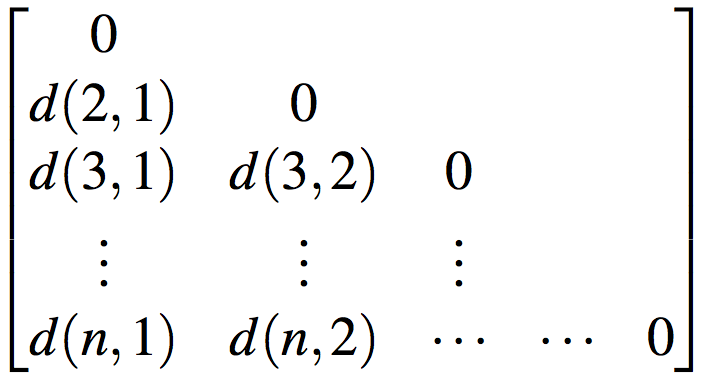
\includegraphics[width=0.3\linewidth]{./figures/matrizdist}
\caption{Estrutura de uma matriz de distâncias. \textit{Retirada de}~\cite{Han2006}}
\label{fig:matriz}
\end{figure}

Tendo existido algumas limitações de \textit{hardware}, mais especificamente da memória do computador, e do tempo de processamento devido ao acesso à base de dados local para obter aos histogramas descritores de cada imagem, optou-se por utilizar o mesmo procedimento utilizado no TweeProfiles~\cite{Cunha2013} e dividir os dados em três partes distintas, resultado em três subconjuntos de 1988 tweets cada. Esta divisão foi efetuada tendo em conta uma divisão temporal, isto é, foi garantido que todos tweets estavam ordenados por ordem cronológica.
 
Para calcular as matrizes de distâncias para o conteúdo visual utilizou-se o histograma descritor de cada imagem, calculando a distância entre histogramas através da função distância Euclidiana apresentada na secção~\ref{subsec:dist}. Assim, resultaram três matrizes distância, cada uma com uma dimensão de $1988 x 1988$.

Com as matrizes distâncias calculadas, estavam reunidas as condições para a integração do modelo no TweeProfiles. O próximo capítulo irá abordar da integração deste modelo com o TweeProfiles e o desenvolvimento da ferramenta Olhó-passarinho e os seus resultados ilustrativos.